\documentclass{beamer}
%
% Choose how your presentation looks.
%
% For more themes, color themes and font themes, see:
% http://deic.uab.es/~iblanes/beamer_gallery/index_by_theme.html
%
\mode<presentation>
{
  \usetheme{default}      % or try Darmstadt, Madrid, Warsaw, ...
  \usecolortheme{default} % or try albatross, beaver, crane, ...
  \usefonttheme{default}  % or try serif, structurebold, ...
  \setbeamertemplate{navigation symbols}{}
  \setbeamertemplate{caption}[numbered]
}

\usepackage[english]{babel}
\usepackage[utf8x]{inputenc}
\usepackage{amsmath}

\title[Kelvin Wave Deep Water Simulation]{Kelvin Wave Deep Water Simulation}
\author{John Meade}
% \institute{Where You're From}
\date{Fall 2015}

\AtBeginSection[]{
  \begin{frame}
  \vfill
  \centering
  \begin{beamercolorbox}[sep=8pt,center,shadow=true,rounded=true]{title}
    \usebeamerfont{title}\insertsectionhead\par%
  \end{beamercolorbox}
  \vfill
  \end{frame}
}

\begin{document}

\begin{frame}
  \titlepage
\end{frame}

% Uncomment these lines for an automatically generated outline.
%\begin{frame}{Outline}
%  \tableofcontents
%\end{frame}

\section{Numerical Methods} %%%%%%%%%%%%%%%%%%%%%%%%%%%%%%%%%%%%%%%%%%%%%%%%%%%%%%%%%%%%%%%%%%%%%%%%%%

\usebackgroundtemplate{
        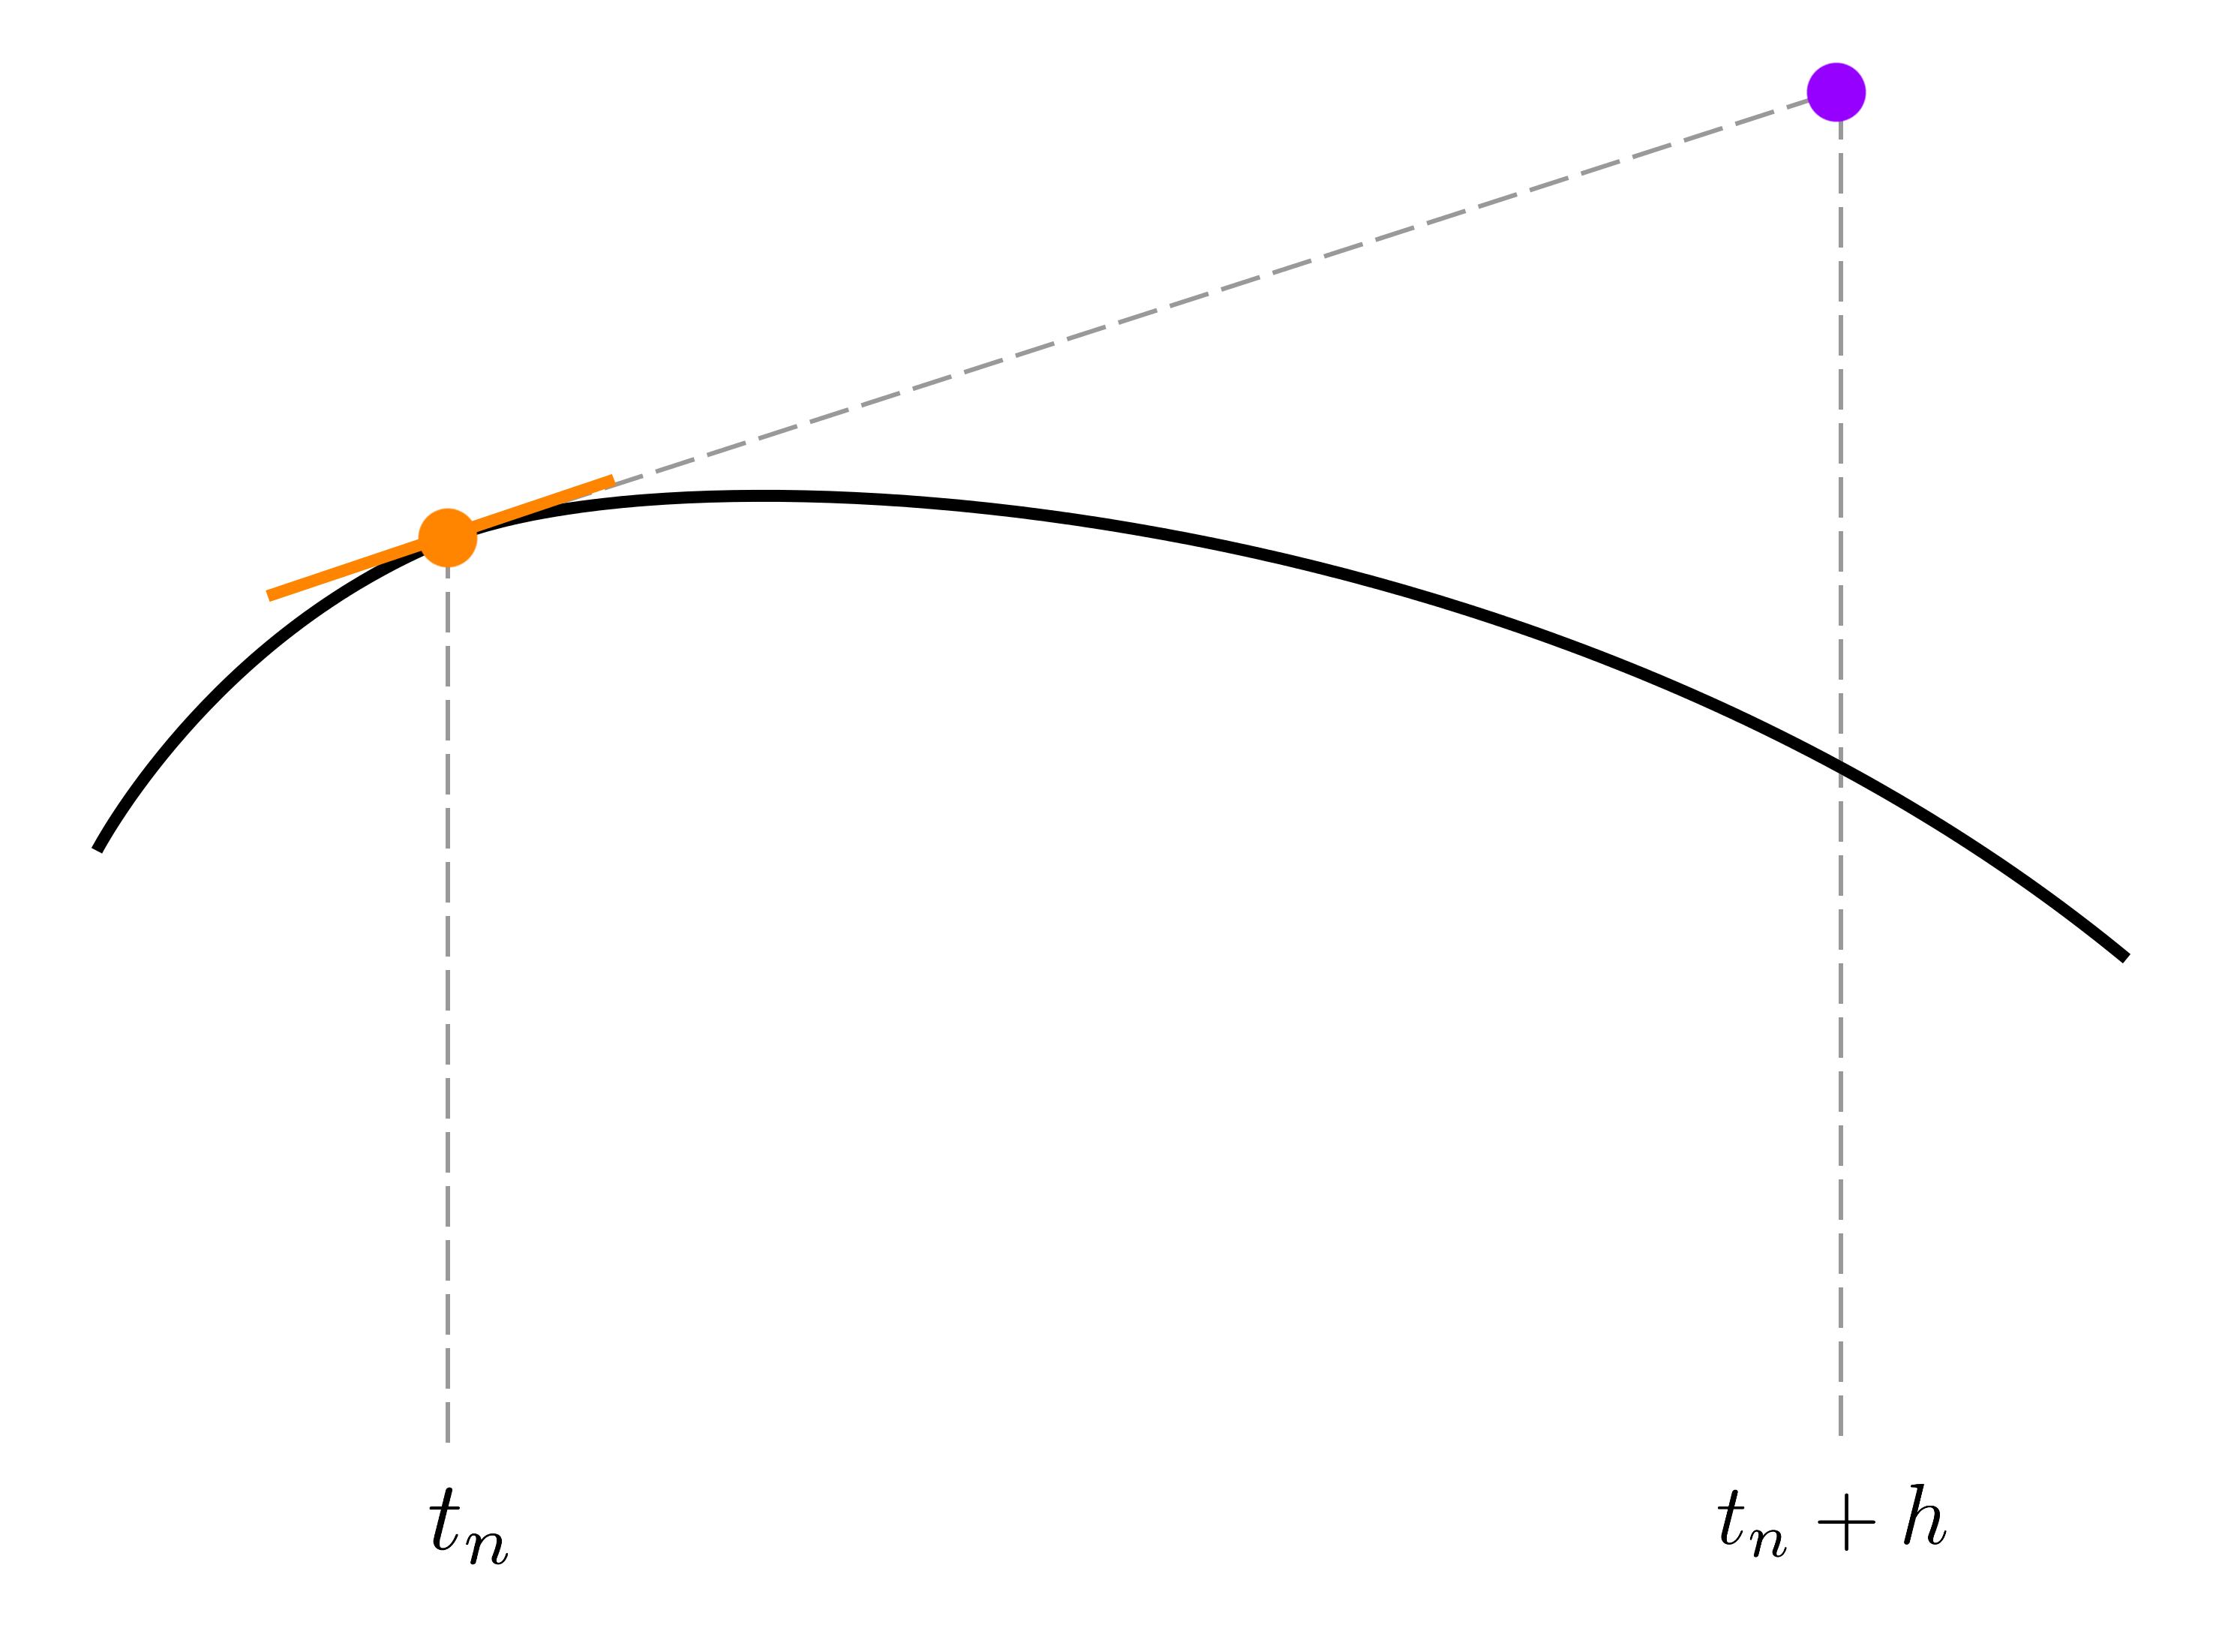
\includegraphics[width=1.2\textwidth]{euler_diagram.png}}
\begin{frame}{Euler Method}

\vspace{0.3\textheight}

$$\textnormal{Let} \:\:\: y = y(t), \:\:\: h \ll 1, \:\:\: f(t,y) = \frac{dy}{dt}$$

% \begin{figure}[h!]
% %   \caption{}
%   \centering
%     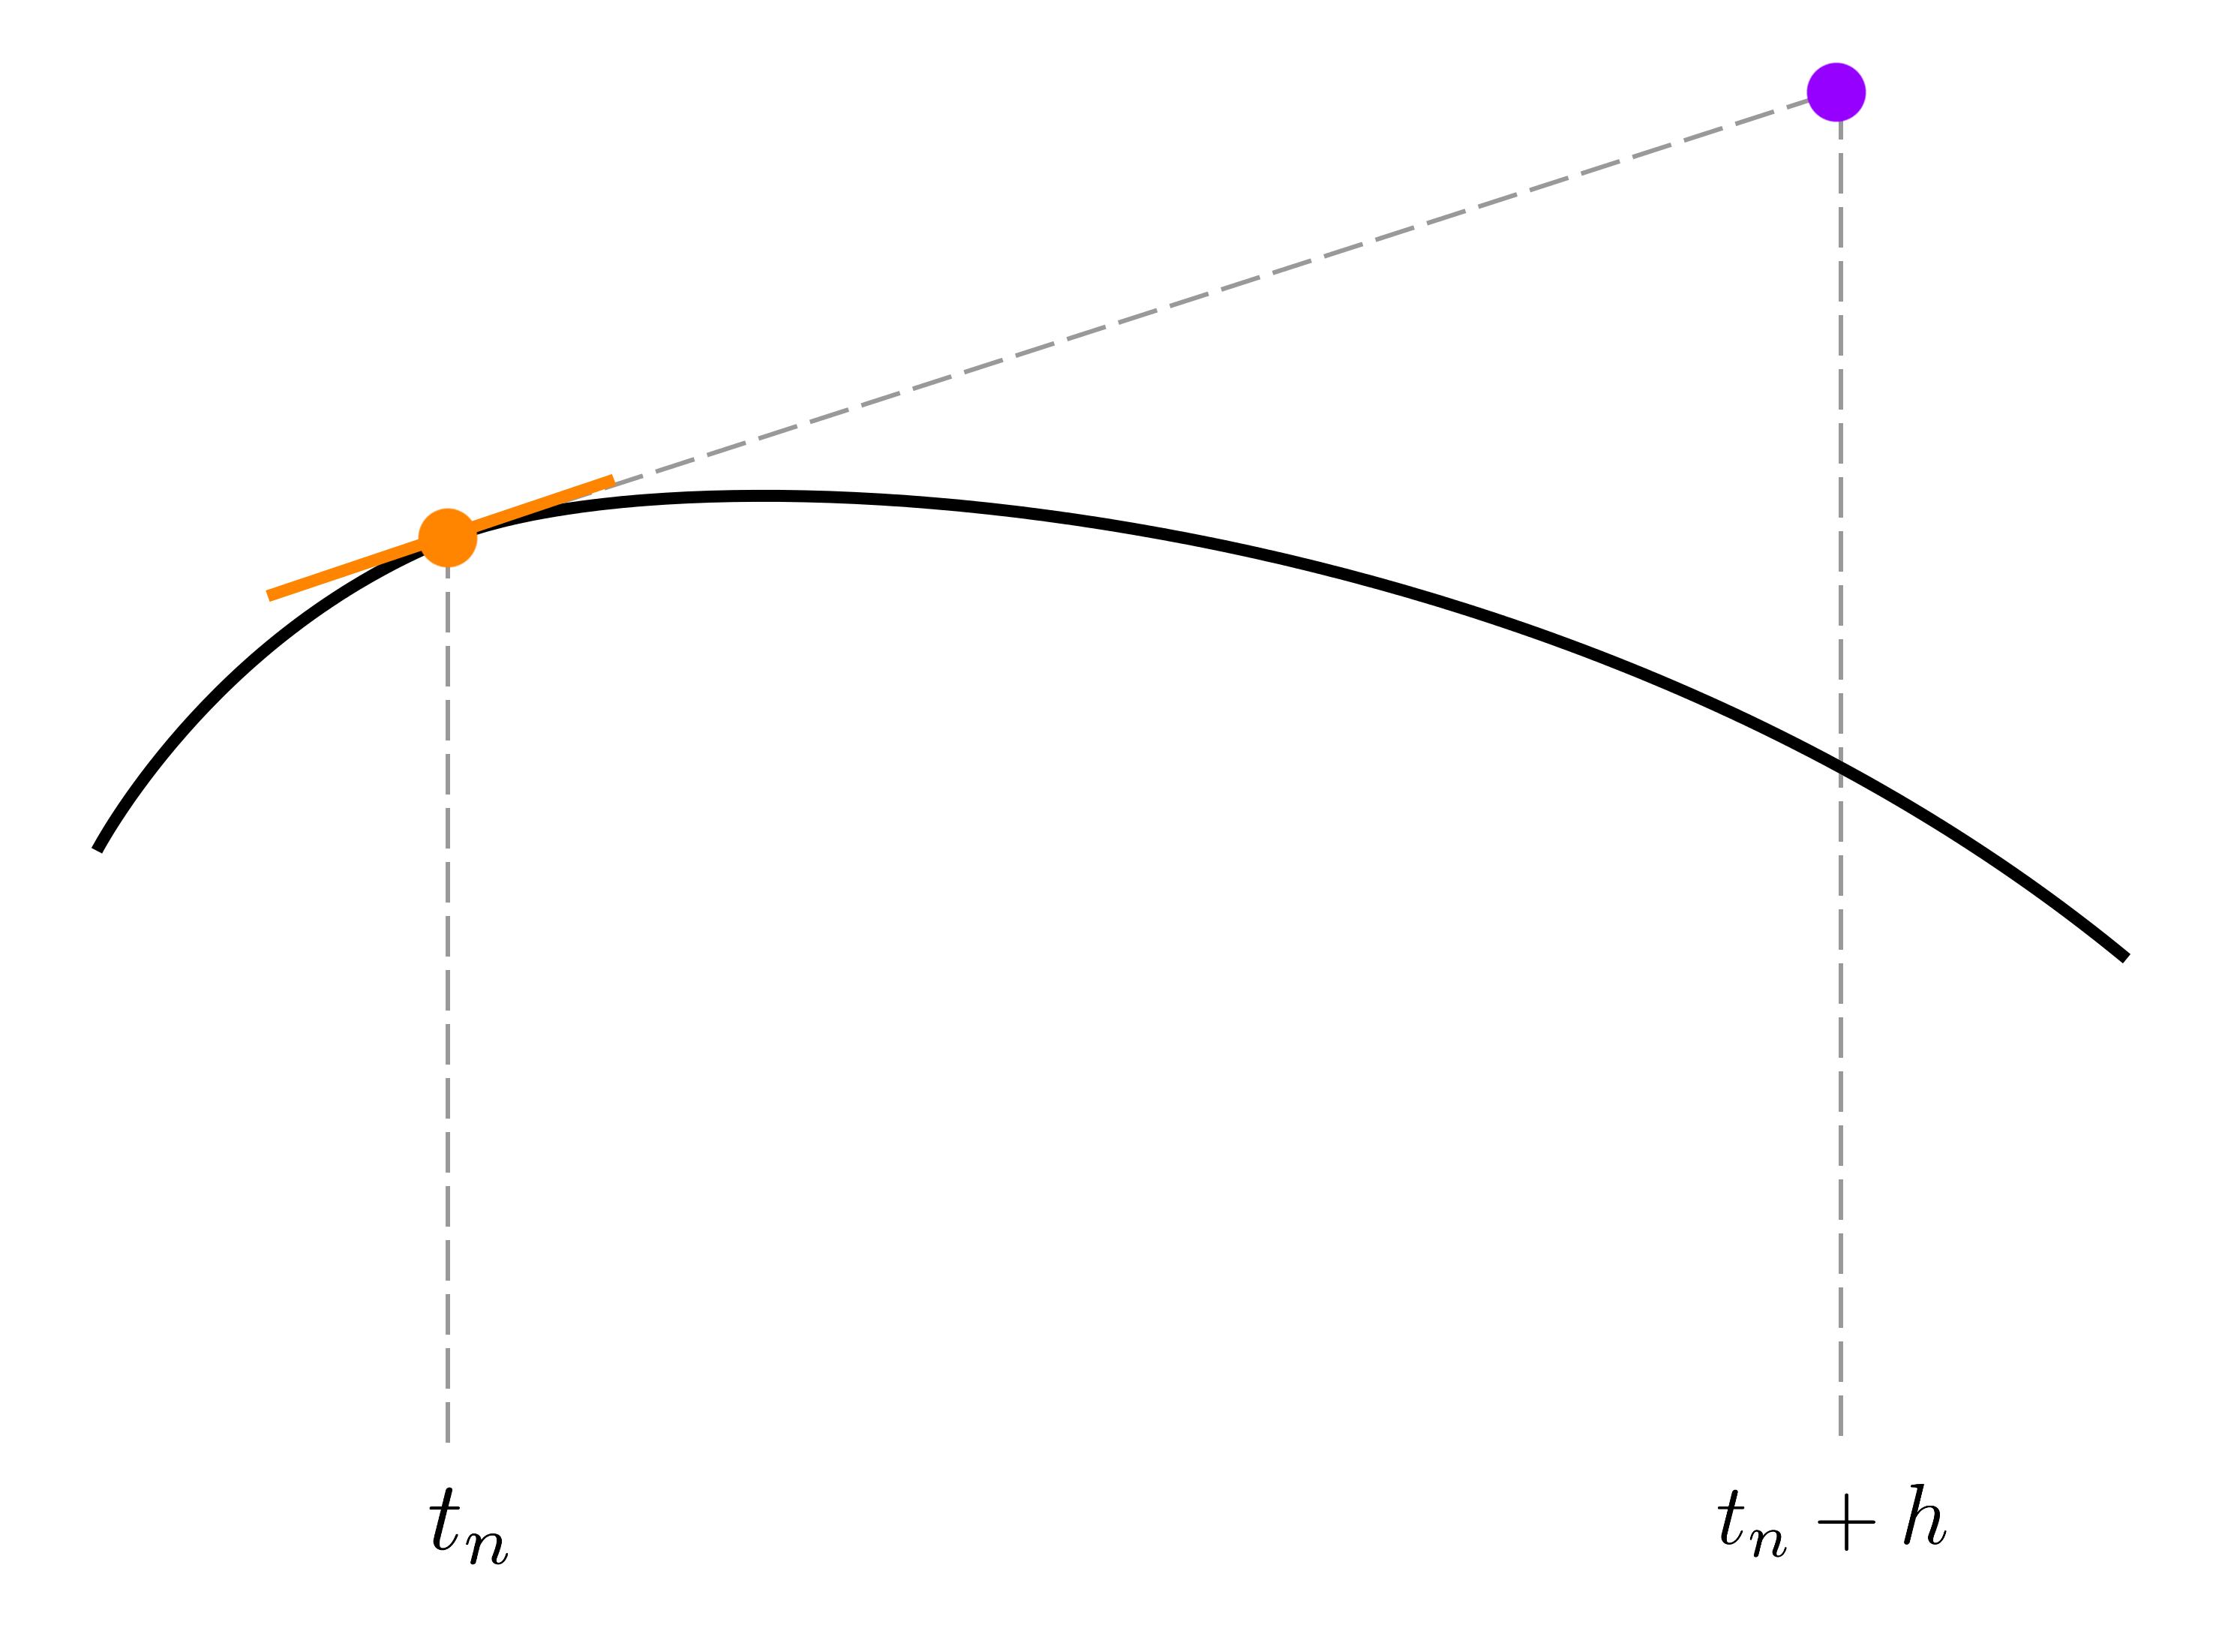
\includegraphics[height=0.6\textheight]{euler_diagram.png}
% \end{figure}

$$f(t,y) \approx \frac{y(t+h) - y(t)}{h}$$

$$\implies y(t+h) \approx y(t) + hf(t,y)$$

% \vskip 1cm

% \begin{block}{Examples}
% Some examples of commonly used commands and features are included, to help you get started.
% \end{block}

\end{frame}

%%%%%%%%%%%%%%%%%%%%%%%%%%%%%%%%%%%%%%%%%%%%%%

\usebackgroundtemplate{}
\begin{frame}{Midpoint Method}

$$y_{n+1}=y_n+h f \left ( t_n+\frac{h}{2}, y_n+ \frac{h}{2} f(t_n,y_n) \right ), \:\:\: f(t,y) = \frac{dy}{dt}$$

\begin{figure}[h!]
%   \caption{}
  \centering
    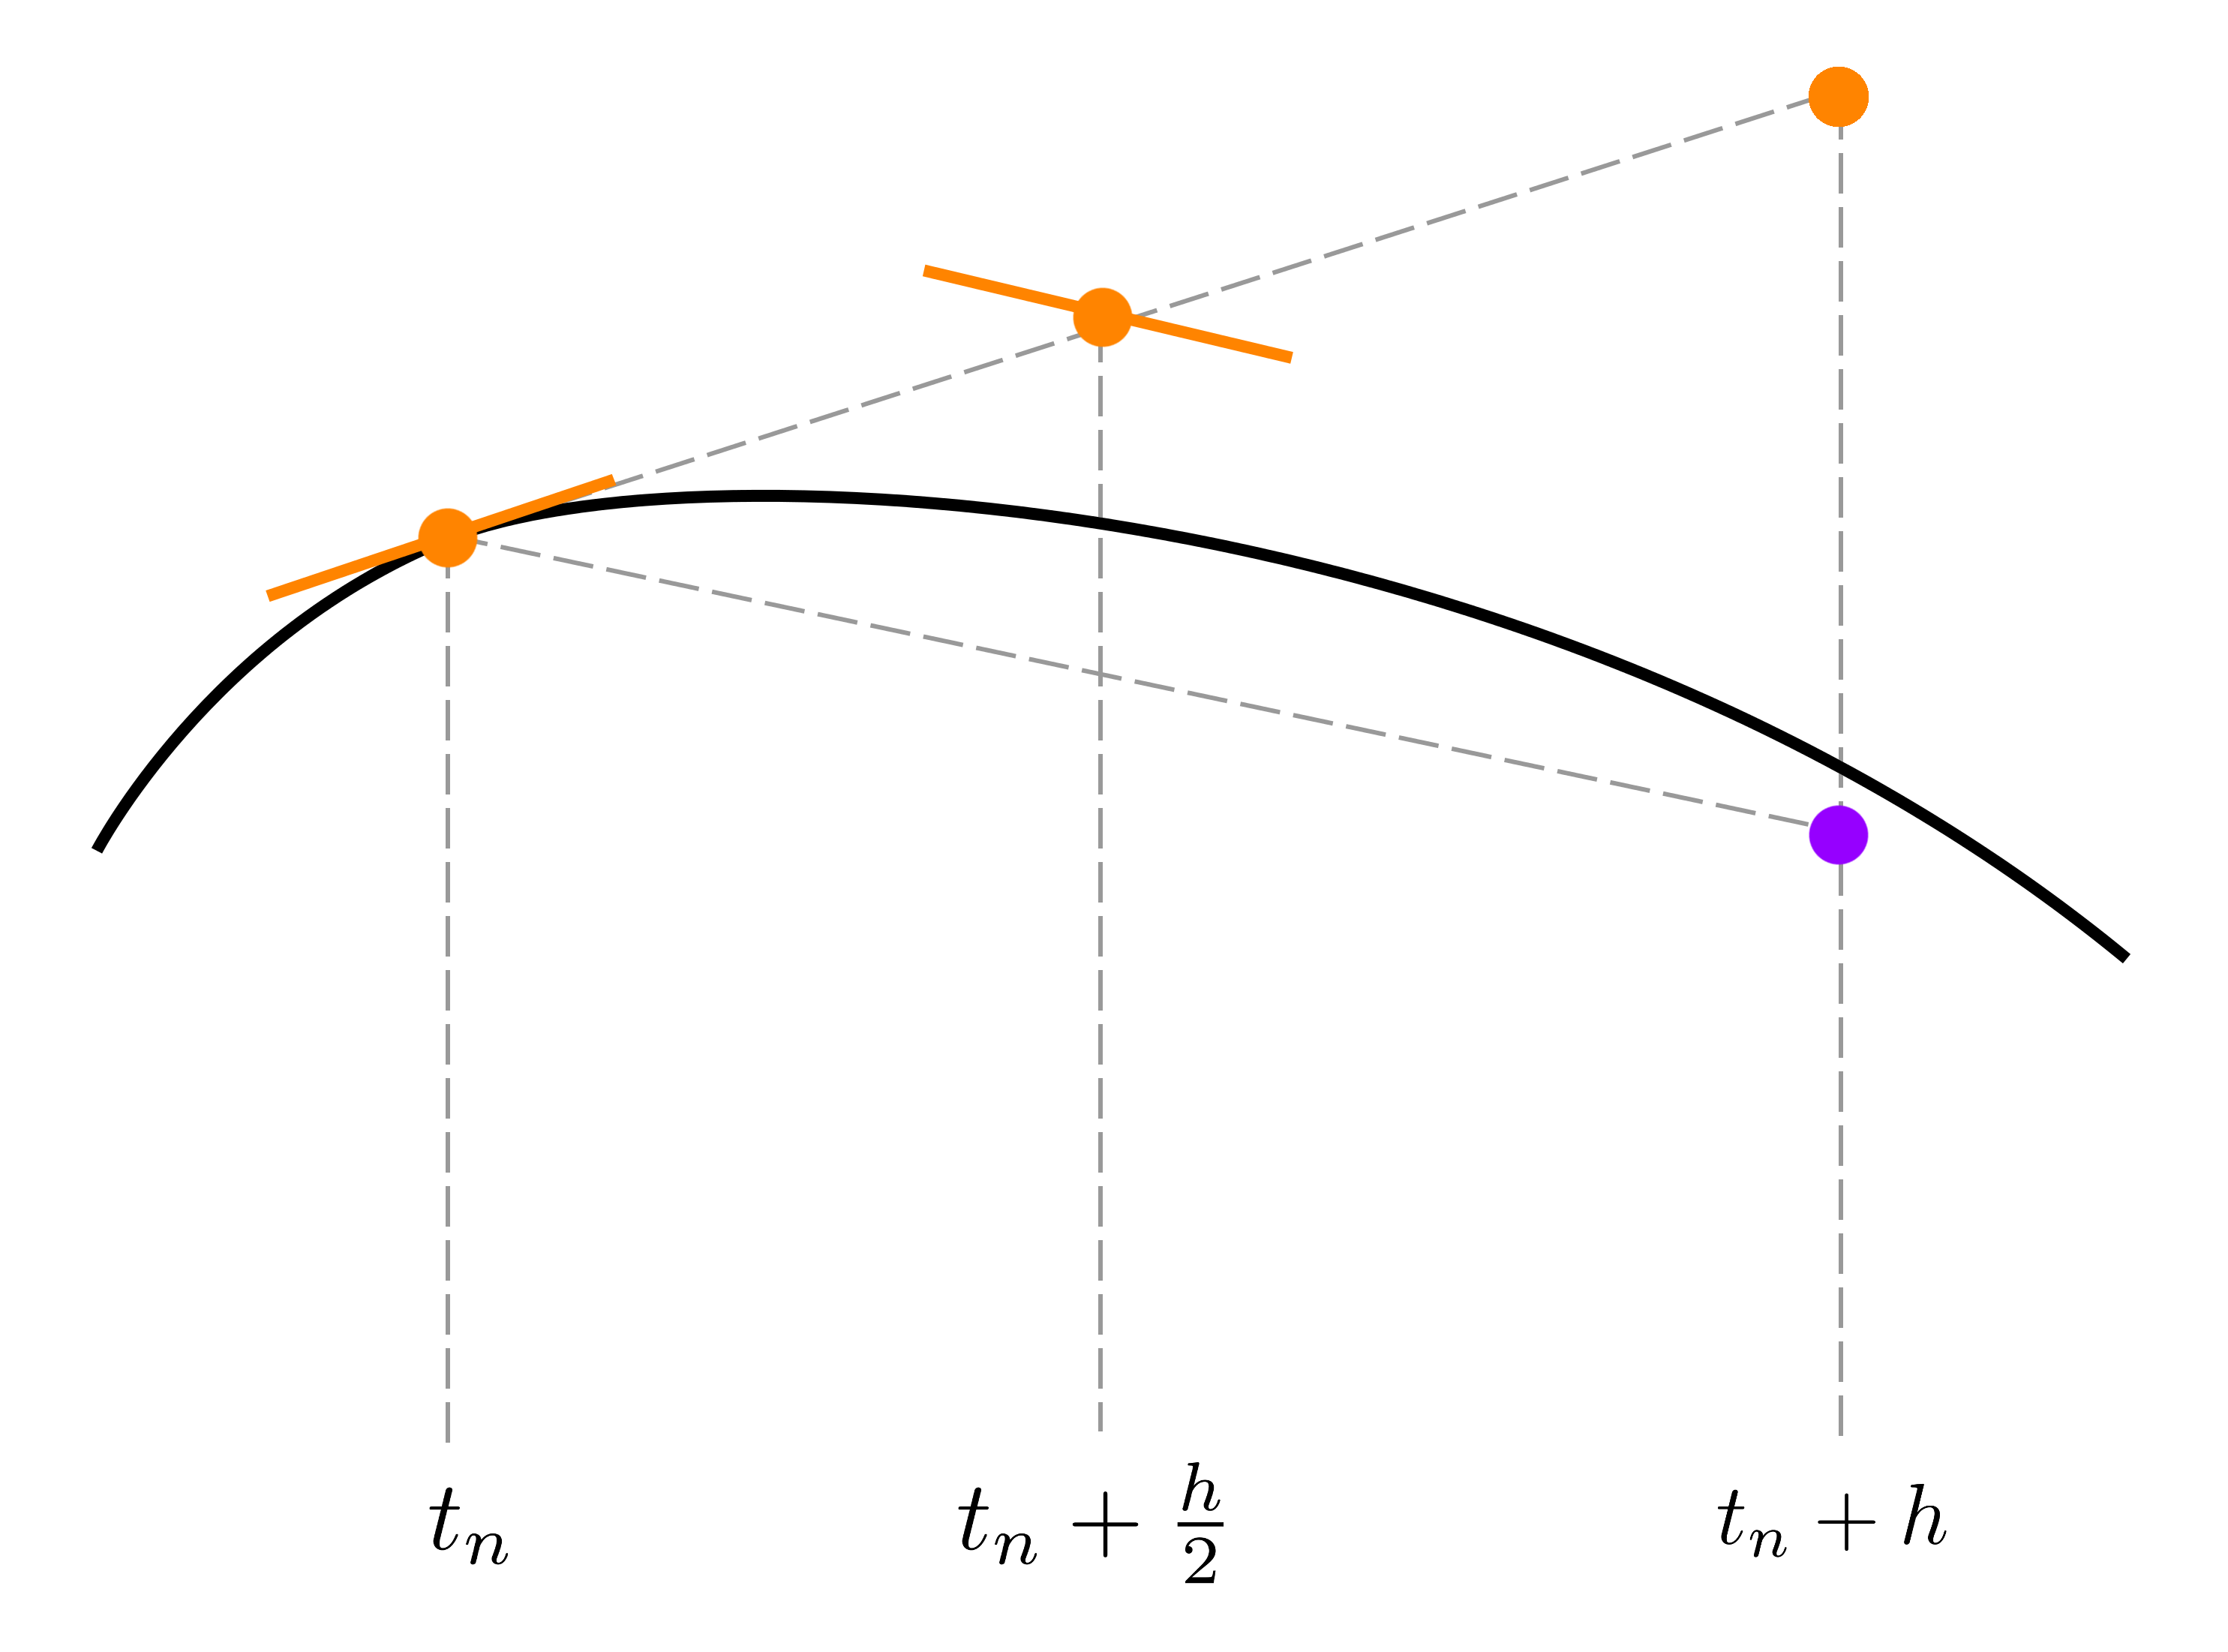
\includegraphics[height=0.7\textheight]{midpoint_diagram.png}
\end{figure}

\end{frame}

%%%%%%%%%%%%%%%%%%%%%%%%%%%%%%%%%%%%%%%%%%%%%%

\usebackgroundtemplate{}
\begin{frame}{Common RK4 Method}

\begin{figure}[h!]
%   \caption{}
  \centering
    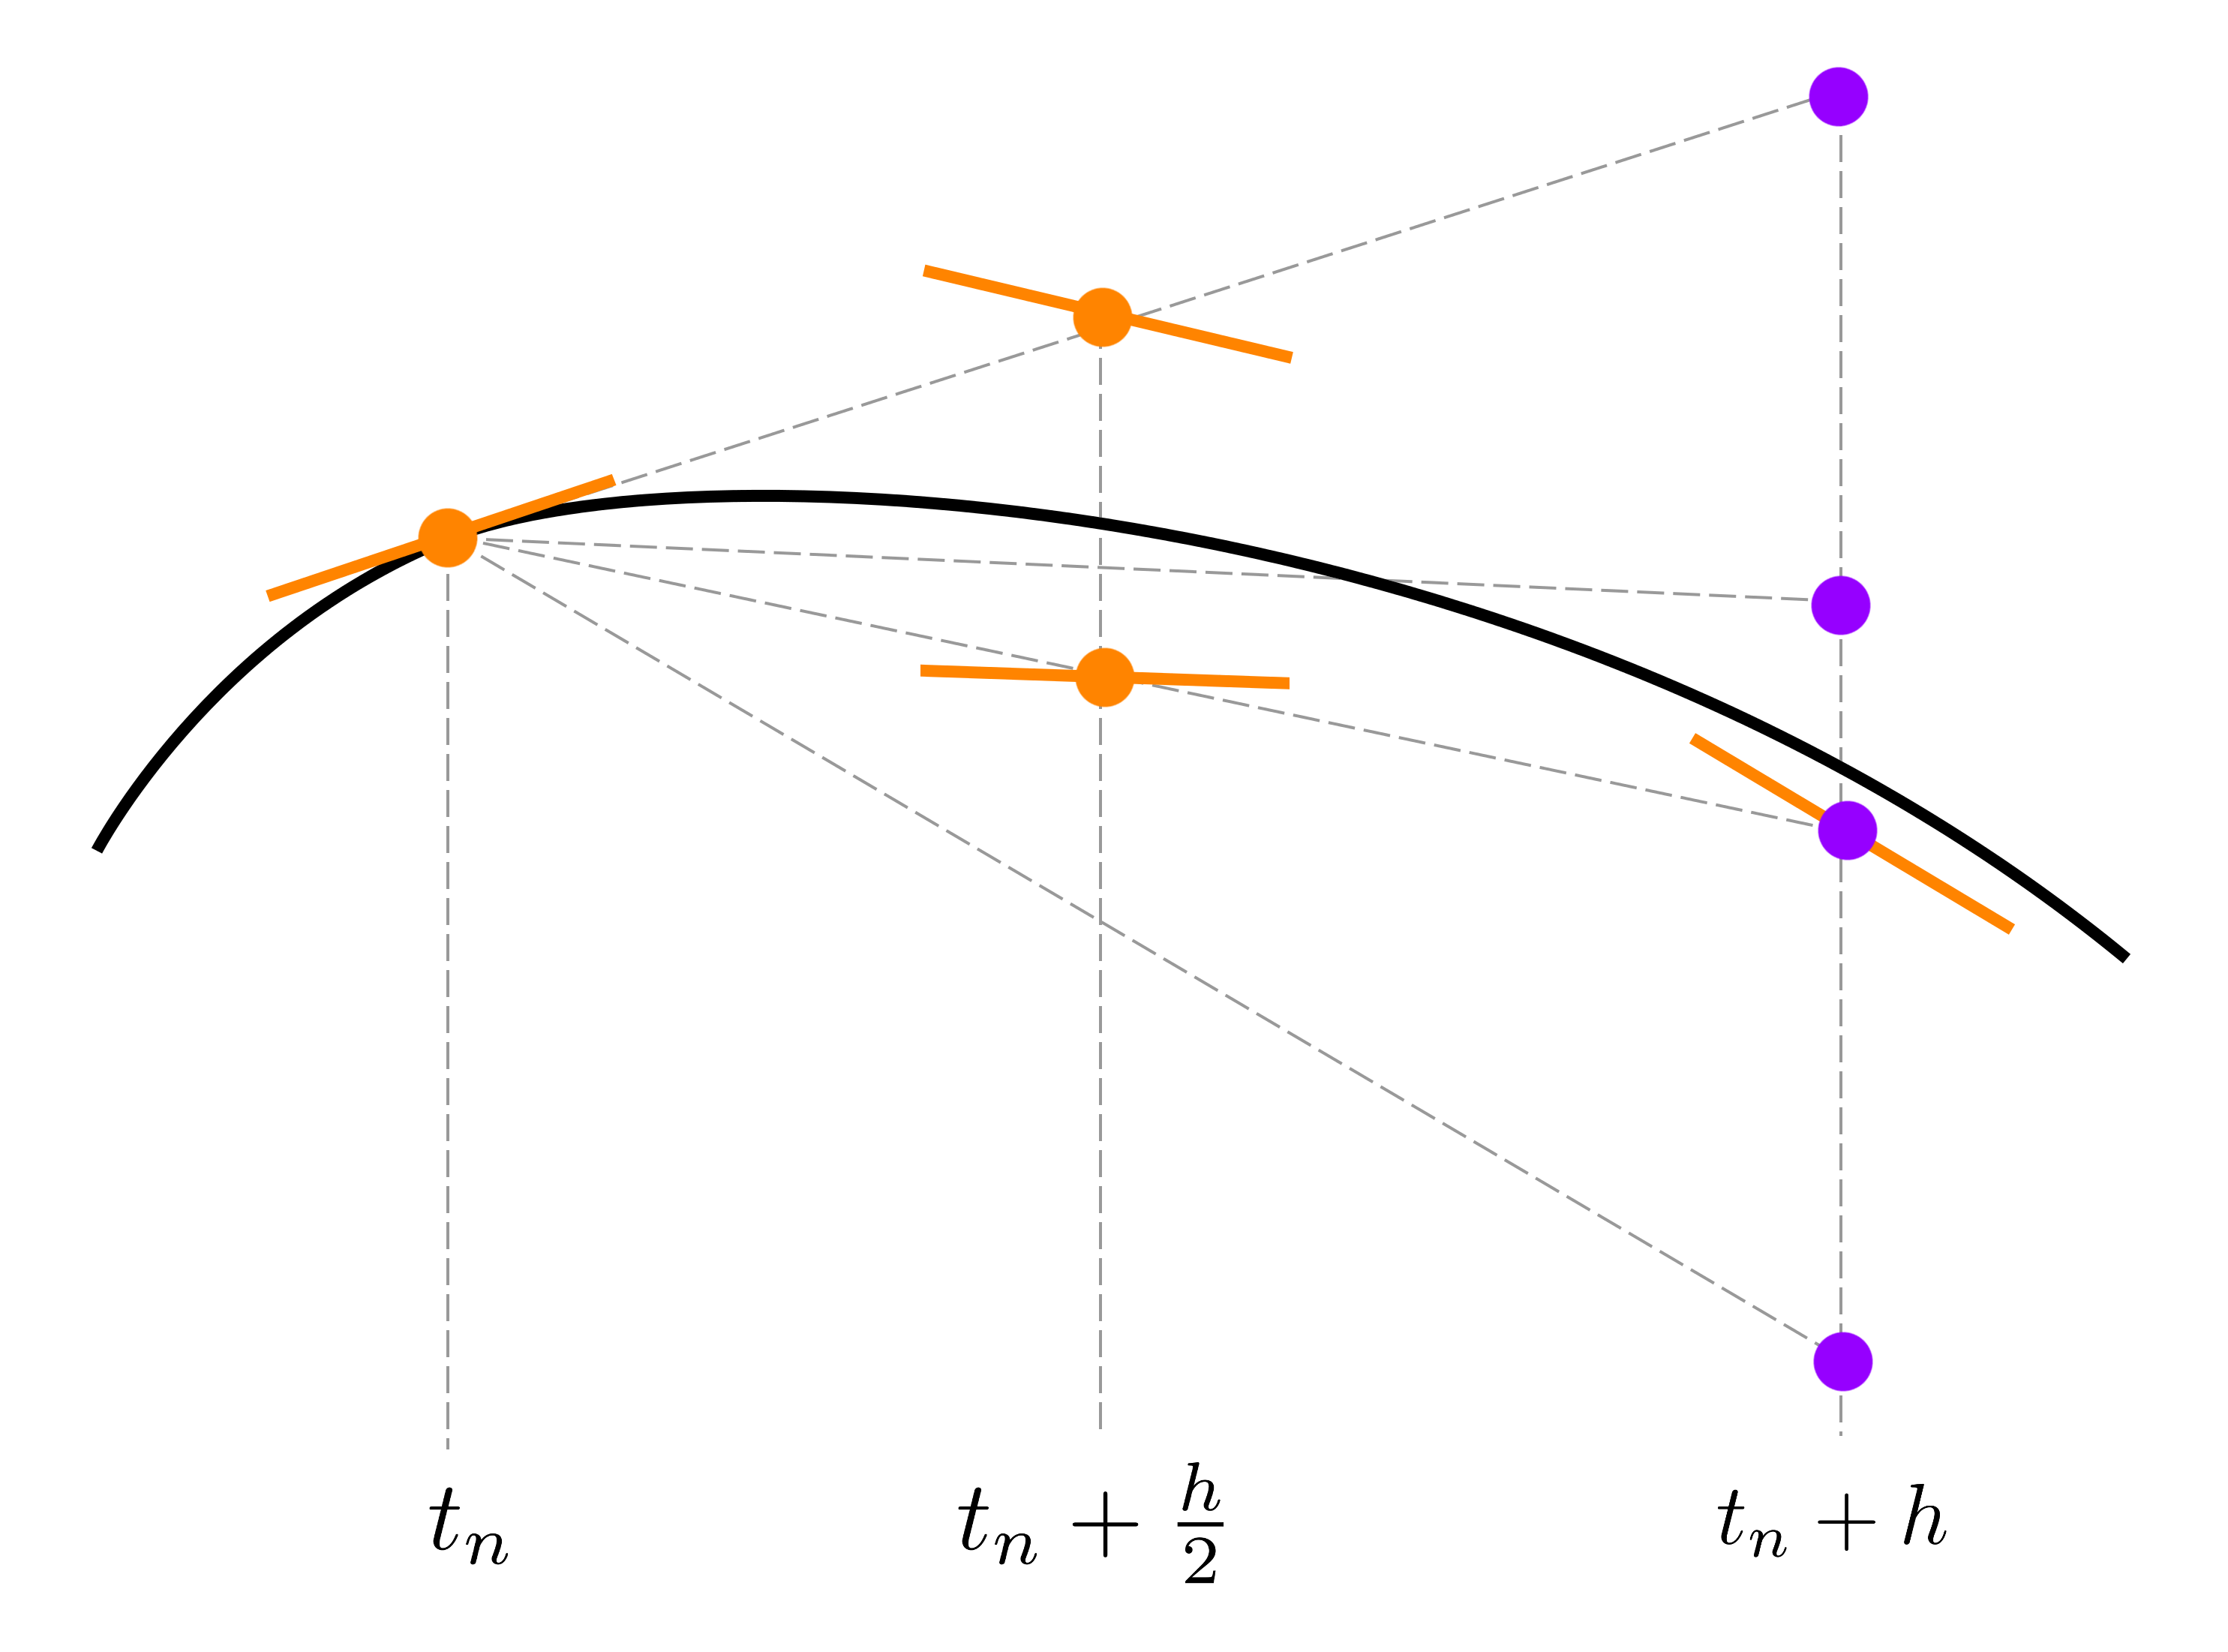
\includegraphics[width=\textwidth]{rk4_diagram.png}
\end{figure}

\end{frame}

%%%%%%%%%%%%%%%%%%%%%%%%%%%%%%%%%%%%%%%%%%%%%%

\setlength{\abovedisplayskip}{0pt}
\setlength{\belowdisplayskip}{0pt}
\setlength{\abovedisplayshortskip}{0pt}
\setlength{\belowdisplayshortskip}{0pt}

\usebackgroundtemplate{}
\begin{frame}{Common RK4 Method}

\begin{columns}

\column{0.5\textwidth}

$$\textnormal{Let} \:\:\: y = y(t), \:\:\: h \ll 1, \:\:\: f(t,y) = \frac{dy}{dt}$$

$$\textnormal{Increment system as follows}$$

\begin{align*}
y_{n+1}&=y_n+\frac{h}{6}(k_1+2k_2+2k_3+k4) \\
t_{n+1}&=t_n+h
\end{align*}

\column{0.4\textwidth}

$$\textnormal{where}$$
\begin{align*}
k_1 &= f(t_n,y_n),\\
k_2 &= f(t_n+\frac{h}{2},y_n+\frac{h}{2}k_1),\\
k_3 &= f(t_n+\frac{h}{2},y_n+\frac{h}{2}k_2),\\
k_4 &= f(t_n+h, y_n+h k_3)
\end{align*}

\end{columns}

\end{frame}

\section{Derivations} %%%%%%%%%%%%%%%%%%%%%%%%%%%%%%%%%%%%%%%%%%%%%%%%%%%%%%%%%%%%%%%%%%%%%%%%%%

\begin{frame}{Kelvin Waves}

(See [1] section 3.8)

\begin{itemize}

\item Assume $u=0$ and $\eta= e^{ly-\sigma t}\phi(x)$

\item Governing equations become
$\begin{cases}
-fv=-g\eta_x \\
v_t=-g\eta_y \\
\eta_t+Hv_y=0
\end{cases}$

\item Solve and obtain
$\eta=\cos(l(y-c_0 t))e^{flx/\sigma}, c_0=\sqrt{gH}$

\end{itemize}

\end{frame}

%%%%%%%%%%%%%%%%%%%%%%%%%%%%%%%%%%%%%%%%%%%%%%%%

\begin{frame}{Deep Water Solution}

(See [1] section 3.3)

\begin{itemize}

\item Kelvin waves assume $u=0$, so consider planar slices parallel to the $yz-$plane

\item In the plane, vorticity has one component, $\omega=w_y-v_z$

\item If $\omega=0$ then $\exists \phi$ such that $v=\phi_y$ and $w=\phi_z$

\item Then $\nabla \cdot (v,z) = 0 \implies \nabla^2 \phi=0$

\item Assume the surface is given by $\eta=a \cos (ky-\sigma t)$ and that the amplitude is small

\item Boundary conditions for surface are $w=\frac{\partial \eta}{\partial t}$ (Las Vagas) and $p=0$ (since water is much denser than air)

\item Bernoulli gives us (assume small velocities, drop quadratic terms) $\frac{\partial \phi}{\partial t}+p+gz=0 \implies \frac{\partial \phi}{\partial t}+g\eta=0$ at $z=0$

\item Try separation of variables, $\phi=f(z) \sin (ky-\sigma t)$

% \item Solve with simplifying assumption that the upper boundary can be considered to be $z=0$ and not $z=\eta$

% \item Assume $\eta$ is small so our boundary conditions can be created for $z=0$ and not $z=\eta$

\end{itemize}

\end{frame}

%%%%%%%%%%%%%%%%%%%%%%%%%%%%%%%%%%%%%%%%%%%%%%%%

\begin{frame}{Deep Water Solution}

After solving, these equations are obtained:

\begin{align*}
\eta (y,t) &= a \cos (ky-\sigma t) \\
v(x,z,t) &= a \sigma e^{kz} \cos (ky-\sigma t) \\
w(x,z,t) &= a \sigma e^{kz} \sin (ky-\sigma t)
\end{align*}

\vspace{0.03\textheight}

The equations of motion for a particle is thus

\begin{align*}
\frac{dy}{dt}&=v(y,z,t) \\
\frac{dz}{dt}&=w(y,z,t)
\end{align*}

\vspace{0.03\textheight}

where a particle path is parameterized by $(y(t),z(t))$.
This is the form needed for Runge Kutta.

\end{frame}

%\section{References} %%%%%%%%%%%%%%%%%%%%%%%%%%%%%%%%%%%%%%%%%%%%%%%%%%%%%%%%%%%%%%%%%%%%%%%%%%

\begin{frame}{References}

[1] Marek Stastna, Aaron Coutino and Michael Waite. (2015). \textit{Fluid Mechanics Notes}

\vspace{0.03\textheight}

[2] PHYS 236, Computational Physics 1 (Fall 2012)

\vspace{0.03\textheight}

[3] Brian P. Flannery, Saul Teukolsky, William H. Press, and William T. Vetterling. (1988). \textit{Numerical Recipes in C: The Art of Scientific Computing}. Cambridge University Press.

\vspace{0.03\textheight}

% [4] \url{https://en.wikipedia.org/wiki/Runge–Kutta_methods}

\end{frame}

\end{document}
